\chapter{She Turned \$1{,}000 Into a \$66M Empire at 76 Years Old!}

This lecture has almost no blackboard mathematics, but it does have a real mathematical spine. We are led from a single realized exit value, to the state changes of persuasion, to a timing comparison between two prices for what Barbara Corcoran insists was the same business, and then all the way back to a \$1{,}000 start, a residential-demand argument, a simple owner-occupant cash-flow identity, and a final rule about beginning with some small but real act of selling. The right way to read the lecture is therefore not as abstract finance, but as a narrated sequence in which arithmetic, strategy, and character slowly lock together.

\section{The \$66 Million Cold Open}

The lecture opens by front-loading the payoff. Barbara Corcoran is stopped on the street and, almost immediately, we are told the number that is meant to organize our attention:
\begin{equation}
V_{\text{exit}}=\$66\,\text{million}.
\end{equation}
The host first asks whether that was the most money she ever made in a year, and she corrects the scale. It was not a year. It was a day. The business was the Corcoran Group, and the money was the sale price that came to her in cash.

That is an important distinction for the notes. The lecture does not begin with a vague notion of wealth. It begins with a realized liquidity event. In that sense, the opening quantity is not paper prestige or an unrealized mark; it is a concrete terminal value.

But the lecture does not stay there. The host quickly rewinds the scene. He tells us that we are in New York, that Barbara is known publicly from \emph{Shark Tank}, and that the point of the interview is not simply to admire the number but to ask how that path was built and what, if anything, can be generalized from it. The rhythm matters. Outcome first, explanation second.

\section{Rejection, Persuasion, and the Operator's Temperament}

Once we are inside the office, the lecture spends a few minutes on banter, style, and competitiveness. Those lines are not disposable. Barbara's speed and appetite for comparison are already on display, and that temper is needed for what follows.

The first serious mechanism comes with the \emph{Shark Tank} story. She says she was chosen, signed, fired, and then recovered the seat before the first day on set. The recovery did not come from waiting politely. It came from writing a vivid email to the producer and arguing that he had made a mistake. She goes further and says that rejection itself had become, in her own life, a lucky charm. In the language of these notes, the lecture is implicitly proposing a simple update rule:
\begin{equation}
\text{rejection}_t \longrightarrow \text{motivation}_{t+1} \longrightarrow \text{assertive response}_{t+2}.
\end{equation}
This is not a law of nature, but it is one of the lecture's recurring dynamics. A negative signal does not terminate the process; it changes the state of the operator.

At the same time, Barbara inserts another lesson which the lecture will later exploit more fully. She says that although she was a phenomenal salesperson and made most of the money in her company that way, the real key to getting ahead was delegation. The line arrives almost casually, but it prepares a second theme: individual selling may start the machine, yet scale demands other people.

The Trump material enters precisely here. Barbara does not praise him for subtlety. She says she learned from him that forceful presentation often carries belief with it, even when the statement is not carefully buttoned up. We should keep the line as her heuristic, not as doctrine. But within the lecture it serves a purpose: it sharpens the contrast between clean truth and effective selling, and it forces the next question.

\section{Sales, Scarcity, and the Hidden Variable}

The host now asks the lecture's first truly operational question: what do we do with a prospect who is on the fence or leaning toward no? Barbara's answer is not a single slogan. It is a mechanism.

\subsection{Question \& Answer}

\paragraph{Question.} How do we move a likely no into a yes?

\paragraph{Answer.} We do not merely keep talking. We alter the state of the deal. Barbara says that she would sometimes take the property away, mention that another buyer had stepped in, or otherwise let scarcity become visible. The prospect, who a moment before was comfortable hesitating, now experiences urgency. At the same time she insists that listening matters more than talking, because the stated desire of the buyer is often not the true motive driving the deal.

\begin{definition}
We shall call the \emph{motivation of a deal} the thing the counterparty is actually trying to maximize or avoid. In this lecture the central warning is that the stated motive and the operative motive are often different.
\end{definition}

That distinction can be written compactly as
\begin{equation}
M_{\text{stated}} \neq M_{\text{true}}.
\end{equation}
Barbara's rough phrase for this is that ``buyers are liars.'' The mathematically cleaner reading is not that every buyer is malicious, but that surface declarations are noisy observations of a hidden variable.

\begin{figure}[h]
\centering
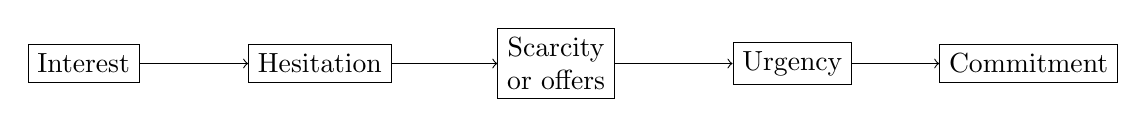
\begin{tikzpicture}
\node[draw, rectangle, align=center] (a) at (0,0) {Interest};
\node[draw, rectangle, align=center] (b) at (3,0) {Hesitation};
\node[draw, rectangle, align=center] (c) at (6,0) {Scarcity\\or offers};
\node[draw, rectangle, align=center] (d) at (9,0) {Urgency};
\node[draw, rectangle, align=center] (e) at (12,0) {Commitment};
\draw[->] (a) -- (b);
\draw[->] (b) -- (c);
\draw[->] (c) -- (d);
\draw[->] (d) -- (e);
\end{tikzpicture}
\caption{Transcript-based reconstruction of Barbara Corcoran's negotiation sequence. The key move is not more explanation but a state change from hesitation to urgency.}
\end{figure}

The lecture's operational claim can therefore be summarized schematically as
\begin{equation}
\text{deal success} \approx f(\text{motivation insight},\ \text{urgency},\ \text{timing}).
\end{equation}
She adds one more ingredient. Listening is not passive. It is diagnostic. One listens not merely to repeat back what the buyer said, but to discover what the buyer will actually move for. That is why Barbara says that if you do not know what is motivating the other person, the rest is guesswork.

\section{Timing and the Same Business at Two Prices}

The lecture then returns to the opening number and asks a sharper question. If Barbara sold the company for \$66 million, what was timing doing in that result? After a brief interruption in the video, the host presses this point directly. Barbara says that she had nearly sold the business one year for only \$2 million and turned the offer down. Two years later, she sold the same business for \$66 million.

We can record the comparison exactly as the lecture gives it:
\begin{align}
V_{\text{early}} &= \$2\,\text{million},\\
V_{\text{late}} &= \$66\,\text{million}.
\end{align}
As a bare scale comparison, and nothing more, this gives
\begin{equation}
\frac{V_{\text{late}}}{V_{\text{early}}}=\frac{66}{2}=33.
\end{equation}

\begin{remark}
This factor of \(33\) is not a full valuation theorem. The transcript does not give earnings, market multiples, capital structure, or any discounted-cash-flow inputs. What it does give is a clear comparative fact: timing changed the price dramatically, even though Barbara herself describes the business as the same business built on the same principle.
\end{remark}

The lecture is refreshingly unromantic here. When asked what she was looking for that made her wait, Barbara does not say she had a subtle market model. She says she was looking for more money. If someone had offered her \$66 million earlier, she would have sold then. That answer is worth preserving because it prevents us from inventing too much mystery. Timing matters, but in this lecture timing is first encountered as bargaining power over an exit, not as a sophisticated macroeconomic forecast.

We can summarize the logic in short derivational form:
\begin{enumerate}
\item An earlier offer existed at \(\$2\) million.
\item The business was not sold at that price.
\item Two years later the business sold at \(\$66\) million.
\item Therefore the same operating asset sat at two radically different prices at two different times.
\item The lecture's conclusion is not ``timing is mystical,'' but ``timing is part of value.''
\end{enumerate}

\section{Real Estate, Vision, and Getting in Early}

After the exit discussion, the lecture walks backward. We are no longer looking at the terminal number; we are looking at the starting condition. The host reminds us that Barbara began with a \$1{,}000 loan:
\begin{equation}
C_0=\$1{,}000.
\end{equation}
When asked for her formula, she does not begin with a spreadsheet. She begins with a vision. She says she saw herself as the queen of New York real estate, that she could see it, touch it, and even knew what color it was. We should not trivialize this. In the lecture the vision functions almost like a boundary condition on action: it determines which motions remain thinkable over long stretches of uncertainty.

The lecture then turns from self-image to market structure. Why residential? Because, Barbara says, people always need a place to live. Through highs and lows in New York, that need persists. This is the closest the lecture comes to a structural demand argument, and it is simple on purpose. The claim is not that housing is riskless, but that residential demand has a baseline that is easier to trust than many more glamorous stories.

\subsection{Question \& Answer}

\paragraph{Question.} What was the formula for accumulating wealth in real estate?

\paragraph{Answer.} The lecture gives a layered answer. First, hold a sufficiently vivid long-run picture of what one is building. Second, choose a segment with persistent demand. Third, enter the game early enough that time can work for you. Fourth, if one is starting with limited capital, structure the first property so that another household helps carry the debt.

That last point is stated very concretely in the interview. Barbara says that if a young person today had about \$100{,}000, she would put it into a two-family house, live in one part, and let the other tenants pay the rent and help pay off the mortgage. In its simplest cleaned-up form, the lecture is invoking the identity
\begin{equation}
C_{\text{owner,net}}
=
C_{\text{mortgage}}+C_{\text{tax}}+C_{\text{upkeep}}-R_{\text{second unit}}.
\end{equation}
This is not a full underwriting sheet. It is the stripped-down point the lecture wants us to see: owner occupancy and tenant rent can be combined so that entry into the asset class is not the same thing as carrying the whole burden alone.

\begin{figure}[h]
\centering
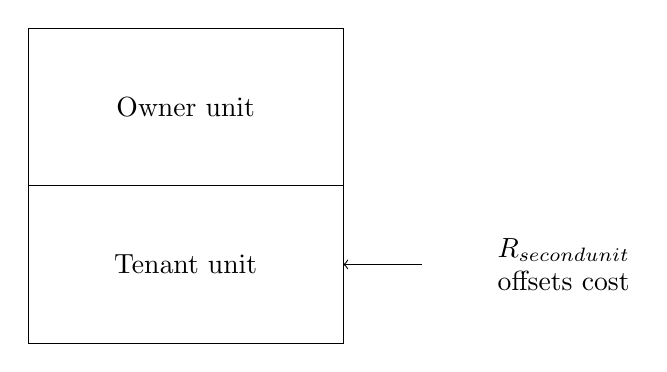
\begin{tikzpicture}
\draw (0,0) rectangle (4,4);
\draw (0,2) -- (4,2);
\node at (2,3) {Owner unit};
\node at (2,1) {Tenant unit};
\draw[->] (5,1) -- (4,1);
\node[align=center] at (6.8,1) {\(R_{\text{second unit}}\)\\offsets cost};
\end{tikzpicture}
\caption{Transcript-based reconstruction of the two-family-house strategy: live in one unit, rent the other, and let the rent reduce the effective carrying cost.}
\end{figure}

Barbara reinforces the importance of early entry by telling a negative story. She once tried to buy a studio in Greenwich Village, became scared, and deliberately failed the board. The cost, in her telling, was about eight years of lost market position:
\begin{equation}
\Delta t_{\text{lost}} \approx 8\ \text{years}.
\end{equation}
That line matters because it translates the lecture's general urge to ``get in the game early'' into a concrete penalty for hesitation.

\section{Concentration, Founder Screening, and Paper Wealth}

The lecture now widens from real estate to investing more generally. The host offers the familiar slogan that concentration builds wealth and diversification keeps it. Barbara immediately resists the slogan. She says she does invest across many businesses, but in practice she is not diversifying by abstract principle; she is judging people. The entrepreneur comes before the sector label.

A useful reconstruction of her screening rule is
\begin{equation}
Q_{\text{investment}}
\approx
f(\text{resilience},\ \text{sales ability},\ \text{judgment},\ \text{fire-in-the-belly}).
\end{equation}
This becomes explicit when she says that the difference between good people and phenomenal people is the ability to get back up. A founder who can rise after being hit is, in the lecture's logic, closer to a sound investment than a pretty business category attached to a weak operator.

The motel story then gives us the chapter's cleanest paper-versus-reality lesson. Barbara says she bought a 12-unit motel. It looked excellent on paper: a nice, juicy rent roll. But when she got inside, she discovered that no one had paid rent in two years. This is exactly the point at which a note-writer should stop trusting the nominal sheet and write down the correction:
\begin{equation}
R_{\text{collected}}=R_{\text{scheduled}}\times \rho_{\text{collection}}.
\end{equation}
In the anecdote, whatever \(R_{\text{scheduled}}\) looked like, the collection rate was effectively close to zero across the relevant horizon. So the true operating cash flow was nowhere near the advertised one.

This is the lecture's sharpest underwriting lesson. A rent roll is not cash. Stated buyer desire is not true motivation. An apparent business category is not yet an investable founder. Again and again the lecture forces us to distinguish surface description from operative reality.

Barbara then says something equally important about losses: she always loses money, and it does not matter in isolation. The game is long. The important thing is not the impossibility of error, but the ability to continue moving through gains and losses without turning either one into an identity crisis.

\section{Doubt, Authenticity, and the First Real Move}

The last section of the lecture becomes broader and more philosophical, but it does not leave business behind. The host asks about where to start today, and Barbara says Pittsburgh: young, educated, full of incoming medical and technology activity, with a local environment friendly to landlords. Then the lecture turns to doubt.

Barbara says she was doubted from the beginning. She names the old boys' club, Donald Trump, and Mark Burnett. One striking numerical marker remains the disputed commission on a Trump property:
\begin{equation}
\Pi_{\text{commission}}=\$4\,\text{million}.
\end{equation}
The exact legal phrasing around that story is rough in the transcript, but the economic point is clear enough: even after doing the work, one may still have to fight for the value one created.

Here the earlier rejection rule returns in mature form. Doubt is not merely endured; it is used. In the lecture's own causal style,
\begin{equation}
\text{doubt}\longrightarrow \text{motivation}\longrightarrow \text{push ahead}.
\end{equation}

The same section also brings in partner choice, poor grades, insecurity, and communication. Barbara says the right life partner or business partner doubles one's chance of success; she says she was not a strong student but was charming; she says insecure people sometimes build very large businesses; and she says that people without affluent parents may in some ways be freer, because they are not under pressure to protect inherited expectations. All of these claims are tied together by one idea: polish is less decisive than the ability to use the assets one actually has.

That is why the lecture ends on authenticity. Barbara says that the moment she became herself, and stopped trying to fit a fancy model, business began to move more cleanly. The closing challenge from the host is extreme: if one started from zero and had one year to make a million dollars, what would one do? Barbara's answer deliberately refuses the grandeur of the question. She says she would sell apples on the corner, make about \$50{,}000 in the first month, and build from there:
\begin{equation}
R_{\text{month 1, apples}}\approx \$50{,}000.
\end{equation}
We should read that not as a literal fruit forecast, but as a final operating rule. Start with something real, something sellable, something that produces cash now. The lecture's last mathematics is therefore the mathematics of motion rather than the mathematics of fantasy.

\section{Summary}

The lecture begins with a terminal value and then patiently walks backward into the machinery that could have produced it. Barbara Corcoran's \$66 million day is not left as a glamorous endpoint. It is decomposed into rejection converted into leverage, sales turned into state changes, timing turned into valuation, residential demand turned into an entry strategy, founder quality turned into an investment filter, and doubt turned into fuel.

What remains after the stories are cleaned up is a compact set of working principles. Surface statements are not the same as true motives. Paper rent is not the same as collected rent. The same business can sit at radically different prices at different moments. Time in the market matters. Founder quality matters. And if we must start from zero, the first honest rule is not to dream about a million dollars; it is to sell something, generate cash, and begin.